\textbf{COLUNI 2024 -- Questão 01}\par\medskip Leia os textos abaixo para responder às questões 1, 2 e 3.

\textbf{Texto I}

\begin{center}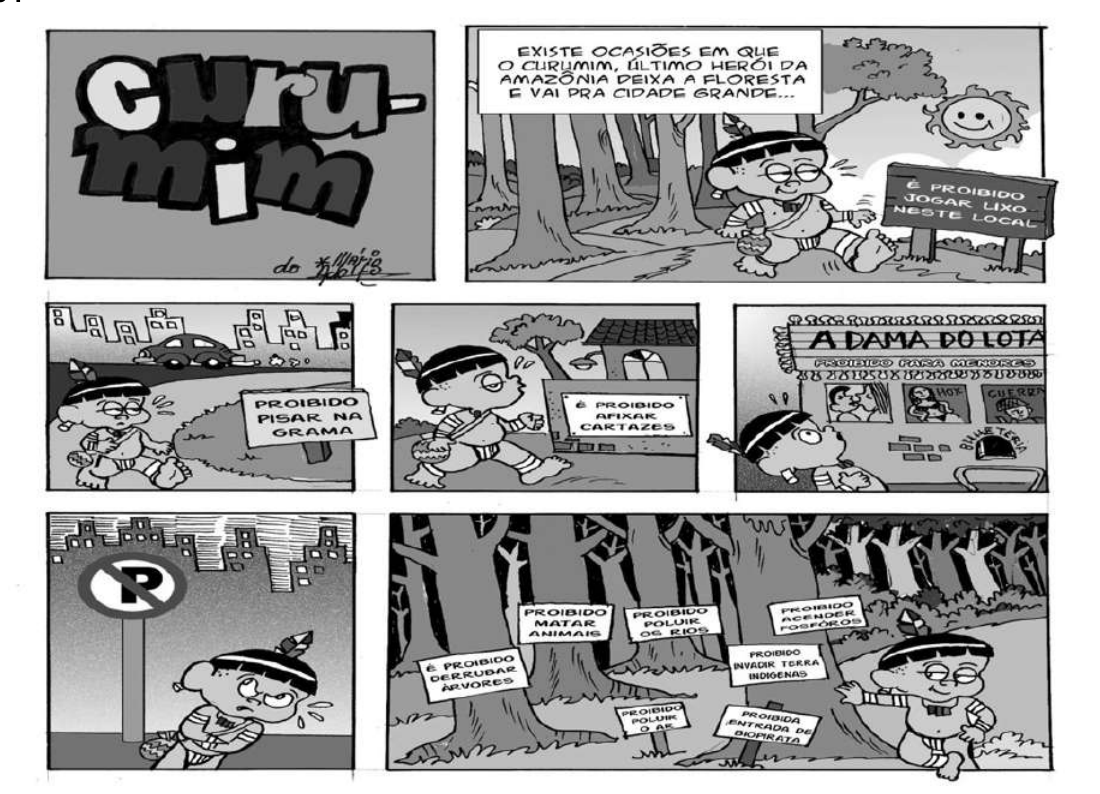
\includegraphics[width=0.90\linewidth]{static/simulados/coluni/figuras/2024/questao-01/figura-1.png}\end{center}
Disponível em: https://marioadolfo.com/festa-na-floresta-curumim-o-ultimo-heroi-da-amazonia-completa-37-anos/. Acesso em: 05 set. 2023.

\textbf{Texto II}

\begin{center}
\includegraphics[width=0.68\linewidth]{static/simulados/coluni/figuras/2024/questao-01/figura-2.png}\end{center}
Disponível em: https://bomjesusdotocantins.pa.gov.br/dia-nacional-de-luta-dos-povos-indigenas/. Acesso em: 19 set. 2023.

Analise as afirmativas abaixo em relação aos textos I e II:

I. Os textos I e II são distintos em relação à prática social exercida, já que o texto I é uma história em quadrinhos e o texto II é um post comemorativo.

II. Os textos, apesar de gêneros textuais distintos, possuem características comuns como a utilização das linguagens verbal e não verbal.

III. Os textos I e II apresentam aspectos composicionais particulares, no que se refere à forma de materializar as informações verbais e não verbais.

IV. O texto I apresenta como característica a função emotiva da linguagem, enquanto, o texto II, a função referencial da linguagem.

Está CORRETO o que se afirma apenas em:
\begin{enumerate}
\item I, II e III.
\item I, III e IV.
\item II, III e IV.
\item I, II e IV.
\end{enumerate}
